%! TeX program = lualatex
%! TEX options = -synctex=1 -interaction=nonstopmode -file-line-error --shell-escape "%DOC%"
\documentclass[10pt,a5paper]{mszalik}

\begin{document}

\thispagestyle{empty}

\begin{center}
	\vspace*{0.5cm}


	\bfseries\scshape
	\huge NIEPOKALANE POCZĘCIE

    \vspace*{0.5cm}

    \huge NAJŚWIĘTSZEJ MARYI PANNY

    \vspace*{0.5cm}

	\vfill

	\begin{figure}[h]
		\centering
		
\includegraphics[width=0.45\linewidth]{logo.png}
	\end{figure}

	\vfill

    \vspace*{0.5cm}

    \bigskip

    {\large Duszpasterstwo Wiernych Tradycji Łacińskiej\\ w Archidiecezji Wrocławskiej}

\end{center}

\newpage

\vspace*{2cm}

\vspace*{\fill}

\hrulefill

{\footnotesize

    Śpiewy i teksty liturgiczne pochodzą z:

	\begin{itemize}[leftmargin=*]
        \item \textit{Zbiór Pieśni nabożnych (Śpiewnik Pelpliński)} (1886),
		\item \textit{Liber Usualis} (1961),
        \item \textit{Monastyczna Liturgia Godzin} (1980),
        \item \textit{ks. Jan Siedlecki -- Śpiewnik kościelny, wydanie XXXIX} (1994),
        \item \textit{Śpiewnik liturgiczny Niepojęta Trójco} (2016),
        \item \textit{ks. Jan Siedlecki -- Śpiewnik kościelny, wydanie XLI} (2021).
	\end{itemize}

	W niektórych przypadkach wykorzystano cyfrową wersję tekstów
	opublikowaną na portalach \textit{brewiarz.pl}, \textit{canocantus.com}, \textit{divinumofficium.com}, \textit{missalemeum.com} i \textit{spiewnik.katolicy.net}.

    \medskip

    Zapis gabc neumów: Piotr Matuszak; Andrew Hinkley et al. \textit{gregobase.selapa.net}.

	\bigskip

	Opracowanie: Mateusz Burszewski, Piotr Matuszak\\
	Skład i łamanie: Michał Siemaszko, Piotr Matuszak\\

    2025, wersja df\\

	\texttt{tradycja.archidiecezja.wroc.pl}
}


%%%%%%%%%%%%%%%%%%%%%%%%%%%%%%%%%%%%%%%%%%%%%%%%%%%%%%%%%%%%%%%%%%%%%%%%%%

\newpage

\fancyhead[CO]{NIEPOKALANE POCZĘCIE NMP}
\fancyhead[CE]{IN CONCEPTIONE IMMACULATA BEATÆ MARIÆ VIRGINIS}

\begin{figure}[h]
    \centering
    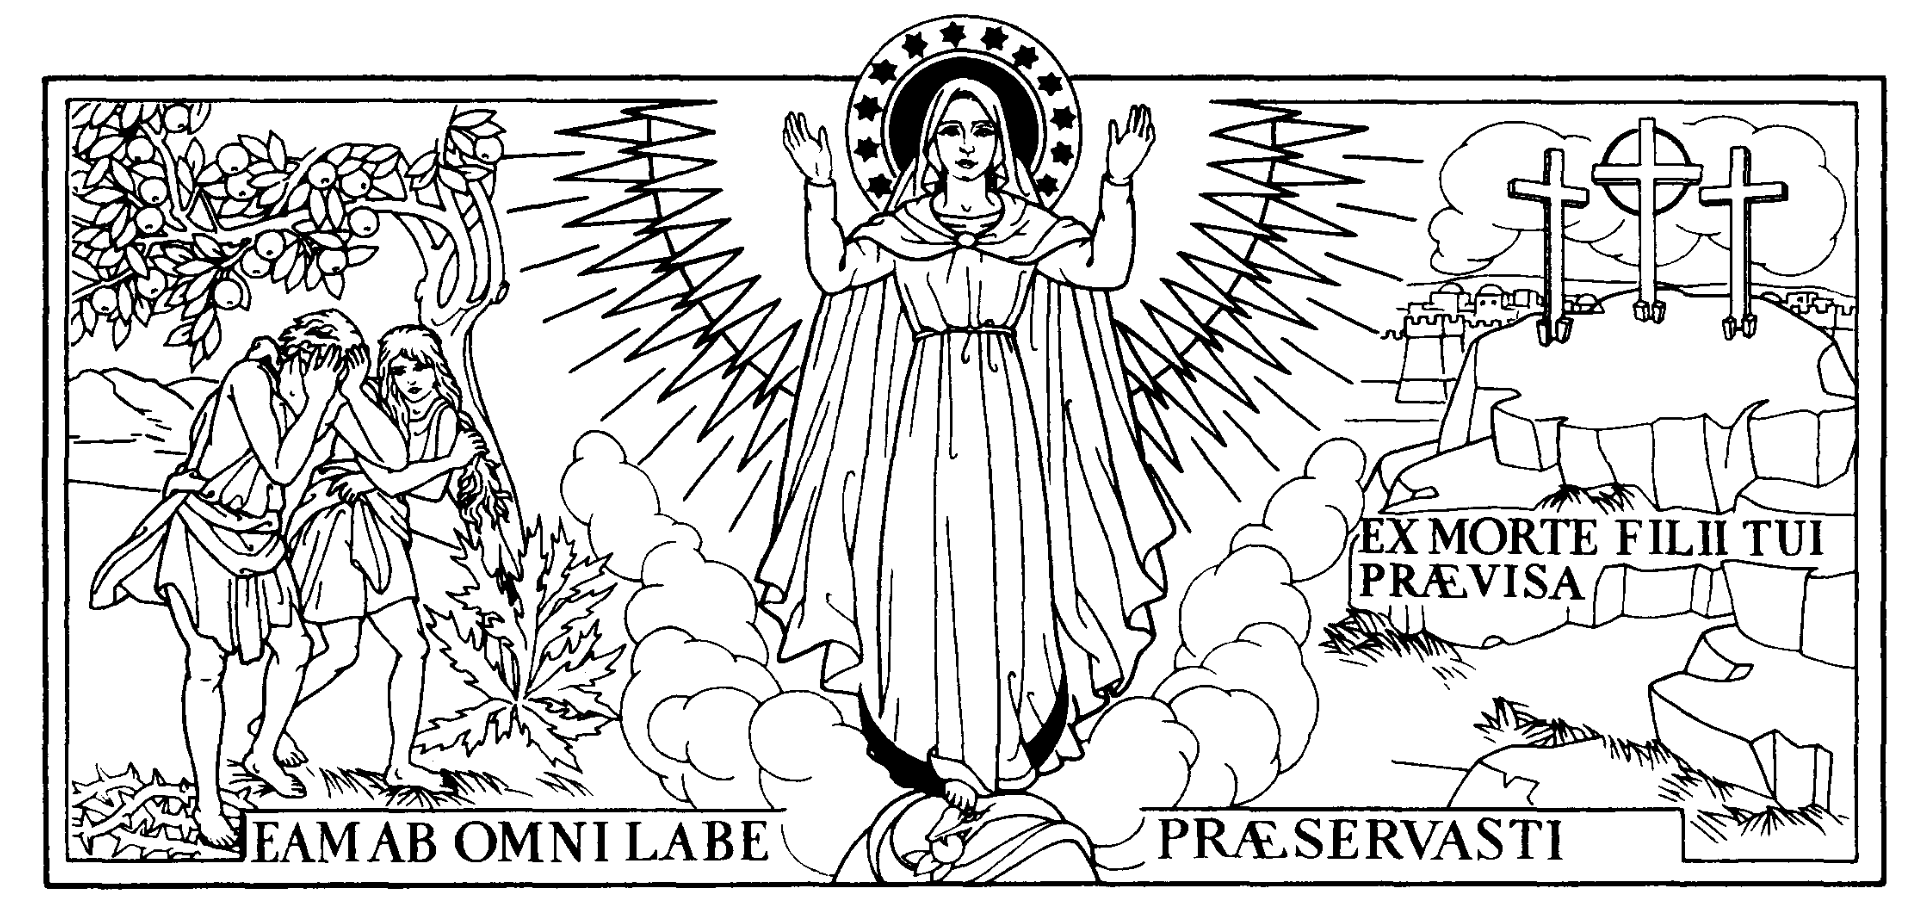
\includegraphics[width=\linewidth]{Figures/in_conceptione_immaculata_bmv_missale_romanum_1962.png}
\end{figure}

\section{MSZA ŚWIĘTA}

\proroctwo{Pieśń}

% \begin{lilypond}
% \relative c' {
%     \key es \major
%     \clef treble
%     \numericTimeSignature
%     \autoBeamOff
%     \time 3/4
%     c4 g'8 g8 f8 es8 d4 c2
%     g'4 bes4 a8 g8 fis4 g2 \break
%     es4 d4 f8 es8 d4 c4.
%     c'8 c4 g2 g4 f8 es8 d4 c2 r4 \bar "|."
% }
% \addlyrics {
%     \override LyricText.font-size = #-1
%         O Mat -- ko mi -- łoś -- ci -- wa,
%         Pan -- no li -- toś -- ci -- wa,
%         Pan -- no u -- ro -- dzi -- wa,
%         Ma -- ry -- a, módl się za na -- mi!
% }
% \end{lilypond}

% \oremuss{
%     \textbf{3.} Tyś świata podziwienie,\\
%     Grzesznych wybawienie,\\
%     Smutnych pocieszenie,\\
%     Marya, módl się za nami!\\

%     \textbf{5.} Nie masz po Bogu w niebie,\\
%     Pewniejszéj krom ciebie\\
%     Nadziei w potrzebie\\
%     Marya, módl się za nami!\\
% }{
%     \textbf{8.} Przez Twe poczęcie czyste,\\
%     I szczęście wieczyste\\
%     Zgotuj nam ojczyste,\\
%     Marya, módl się za nami!\\

%     \textbf{10.}  Zjednaj nam zlitowanie,\\
%     Z tobą królowanie,\\
%     Dajże nam to, Panie.\\
%     Marya, módl się za nami!\\
% }

\begin{lilypond}
\relative c' {
    \key d \major
    \clef treble
    \autoBeamOff
    \time 4/4
    a'2 b2 a4 a4 g4 b4 a4[(g4)] fis2
    a2 b2 a4 a4 g4 b4 a4[(g4)] fis2
    fis4 fis4 e4 e4 a4 a4 g4 g4
    fis4 fis4 e4 e4 a4 a4 g4 b4
    a2 g2 fis1 \bar "|."
}
\addlyrics {
    \override LyricText.font-size = #-1
        Mat -- ko nie -- bies -- kie -- go  Pa -- na,
        ślicz -- naś i Nie -- po -- ka -- la -- na,
        ja -- kiej wie -- ki, czas da -- le -- ki,
        czas nie -- ma -- ły i świat ca -- ły nie sły -- szał.
}
\end{lilypond}

\oremuss{
    \textbf{2.} Wszystkie skarby, co są w niebie,\\
    wydał, Panno, Bóg dla Ciebie:\\
    jak bogata słońca szata,\\
    z gwiazd korona upleciona\\
    na głowie.
}{
    \textbf{3.} Miesiąc swe ogniste rogi\\
    skłonił pod Twe święte nogi;\\
    gwiazdy wszystkie asystują,\\
    bo Królową w niebie czują\\
    nad sobą.
}

\oremusmidadj{1cm}{
    \textbf{4.} Przez poważną Twą przyczynę\\
    niech nam Bóg odpuści winę.\\
    Uproś pokój, Panno Święta,\\
    boś bez zmazy jest poczęta,\\
    Maryjo!
}

\newpage

\oremus{Introit (Iz 61:10; Ps 29:2)}{
    Gaudens gaudébo in Dómino, et exsultábit ánima mea in Deo meo:
    quia índuit me vestiméntis salútis: et induménto justítiæ circúmdedit me,
    quasi sponsam ornátam monílibus suis.\\

	Exaltábo te, Dómine, quóniam suscepísti me: nec delectásti inimícos meos super me. \medskip

	Glória Patri\dots \\

    \textit{Gaudens gaudébo\dots}
    }{
    Weselę się wielce w Panu i raduje się duch mój w moim Bogu:
    gdyż oblókł mnie w szaty zbawienia i odział płaszczem świętości
    jak oblubienicę ubraną klejnotami.\\\\

    Sławić Cię będę, Panie, bo mnie wybawiłeś i nie sprawiłeś ze mnie uciechy mym wrogom.\medskip

	Chwała Ojcu\dots\\

    \textit{Weselę się\dots}
}

\bigskip

\grecommentary[0.15cm]{Missa Cum iubilo (IX)}
\gregorioscore{Melody/ky--kyrie_ix--solesmes.1.gabc}

\newpage

\grechangestaffsize{15}
\grecommentary[0.15cm]{Missa De Angelis (VIII)}
\gregorioscore{Melody/ky--gloria_viii--solesmes.1.gabc}
\grechangestaffsize{17}

\newpage

\oremus{Kolekta}{
    Deus, qui per immaculátam Vírginis Conceptiónem dignum Fílio tuo habitáculum præparásti:
    quǽsumus; ut, qui ex morte ejúsdem Filii tui prævísa eam ab omni labe præservásti,
    nos quoque mundos ejus intercessióne ad te perveníre concédas. Per eúndem\dots
}{
    Boże, któryś przez Niepokalane Poczęcie Najświętszej Dziewicy przygotował Synowi Swojemu
    godne mieszkanie, prosimy Cię: jak na mocy zasług przewidzianej śmierci tegoż Syna Twego zachowałeś
    Ją od wszelkiej zmazy, tak dozwól nam za Jej przyczyną dojść do Ciebie czystymi.
    Przez tegoż Pana\dots
}

\oremus{Kolekta (wspomnienie dnia Adwentu)}{
    \vspace{-4pt}
    Excita, Dómine, corda nostra ad præparándas Unigéniti tui vias:
    ut, per ejus advéntum, purificátis tibi méntibus servíre mereámur:
    Qui tecum\dots
}{
    \vspace{-4pt}
    Pobudź, Panie, serca nasze do gotowania dróg Jednorodzonemu Synowi Twemu,
    abyśmy dzięki Jego przyjściu mogli Ci służyć oczyszczoną duszą.
    Który z Tobą\dots
}

\proroctwo{Lekcja (Prz 8:22-35)}

Wyjątek z Księgi Przysłów

Pan posiadł mnie na początku dróg swoich, zanim cokolwiek od początku uczynił. 
Od wieków zrządzona jestem i od starodawna, zanim ziemia powstała. 
Nie było jeszcze przepaści, a jam poczęta była. 
Jeszcze nie wytrysnęły źródła wód, jeszcze ciężarem swym nie stanęły góry: 
przed pagórkami jam była zrodzona. 
Jeszcze nie uczynił był ziemi ni rzek, ni zawias okręgu ziemi. 
Gdy niebiosa urządzał, byłam przy tym: 
gdy nad przepaścią krąg ziemski utwierdzał, 
gdy w górze umacniał niebiosa i w karby ujmował źródła wód, 
gdy morzu zakreślał granice jego i wodom nadawał prawo, by nie przekraczały swych granic, 
gdy ziemię ustalał w posadach. 
Z Nim byłam wszystko wespół urządzając i radowałam się na każdy dzień, igrając ciągle przed Jego obliczem, 
igrając na ziemskim okręgu — a rozkosz moja przebywać wśród synów ludzkich. 
Teraz więc, synowie, słuchajcie mnie: Błogosławieni, którzy strzegą dróg moich. 
Słuchajcie nauki, a bądźcie mądrzy i nie od rzucajcie jej. 
Błogosławiony człowiek, który mnie słucha i który czuwa co dzień u drzwi moich i strzeże podwojów mej bramy. 
Kto mnie znajdzie, znajdzie życie i wyczerpie zbawienie od Pana.

\oremus{Graduał (Jdt 13:23, 15:10)}{
    Benedícta es tu. Virgo María, a Dómino, Deo excélso, præ ómnibus muliéribus super terram.

    Tu glória Jerúsalem, tu lætítia Israël, tu honorificéntia pópuli nostri.
}{
    Błogosławiona jesteś, Panno Maryjo, od Pana, Boga, wysokiego, ponad wszystkie niewiasty na ziemi.

    Tyś chwałą Jeruzalem, Tyś weselem Izraela, Tyś chlubą ludu naszego.
}

\newpage

\oremus{Alleluja (Pnp 4:7)}{
    Allelúja, allelúja. Tota pulchra es, María: et mácula originális non est in te. Allelúja.
}{
    Alleluja, alleluja. Cała piękna jesteś, Maryjo, i zmazy pierworodnej nie ma w Tobie. Alleluja.
}

\proroctwo{Ewangelia (Łk 1:26-28)}

Ciąg dalszy \ding{64} Ewangelii według Łukasza.

Onego czasu: Posłany jest Anioł Gabriel od Boga do miasta galilejskiego, które zwano Nazaret,
do Panny poślubionej mężowi, któremu było na imię Józef, z domu Dawidowego, a imię Panny Maryja.
I wszedłszy do Niej Anioł rzekł: «Bądź pozdrowiona, łaski pełna, Pan z Tobą, błogosławionaś Ty między niewiastami».


\bigskip 

% \vfill

% \centerline{\pgfornament[width=7cm]{82}}

% \vfill

% \newpage

\grechangestaffsize{16}
\grecommentary[0.15cm]{Credo (IV)}
\gregorioscore{Melody/ky--credo_iv--solesmes.1.gabc}
\grechangestaffsize{17}

\newpage

\oremus{Ofertorium (Łk 1:28)}{
    Ave, María, grátia plena; Dóminus tecum: benedícta tu in muliéribus, allelúja.
}{
    Zdrowaś Maryjo, łaski pełna, Pan z Tobą, błogosławionaś Ty między niewiastami, alleluja.
}

\proroctwo{Pieśń}

\begin{flushright}
\footnotesize{\textit{melodia: XVII w., staniątecka}}
\end{flushright}

\vspace{-10pt}

\begin{lilypond}
\relative c' {
    \clef treble
    d2 a'8[(g8)] a8[(b8)] c4 d4.(c8) b8[(a8)] b2 a2
    a2 f4 g4 a4 g4.(f8) e8([d8]) e2 d2 \break
    f2 f4 g4 a4 bes4.(a8) g8[(f8)] g2 a2
    e2 f4 g4 a4 g4.(f8) e8[(d8)] e2 d2 \bar "|."
}
\addlyrics {
    \override LyricText.font-size = #-1
    Gwiaz -- do mo -- rza głę -- bo -- kie -- go,
    Mat -- ko Bo -- ga naj -- wyż -- sze -- go:
    Pa -- nien -- ko, bądź po -- zdro -- wio -- na,
    Fór -- to raj -- ska o -- two -- rzo -- na.
}
\end{lilypond}

\oremuss{
    \textbf{2.} Od Aniołaś pozdrowiona,\\
    Gdyś poczęła w sobie Pana;\\
    Imię Matki naszéj owéj\\
    Odmieniaj ku pokojowi.\\

    \textbf{3.} Rozwiąż związki zadłużonym,\\
    Przynieś światło zaślepionym:\\
    Odpędź od nas, co jest złego,\\
    daj chcieć i mieć, co dobrego.\\

    \textbf{4.} Iżeś Matka, niech poznamy;\\
    Gdy się więc modlisz za nami,\\
    Niechaj cię Syn twój wysłucha,\\
    Ku nam grzesznym skłoni ucha.\\
}{
    \textbf{5.} Panno we wszém osobliwa,\\
    Skromna, cicha i cierpliwa,\\
    Odproś nasze wszystkie winy,\\
    Uczyń z grzesznych Boże syny. \\

    \textbf{6.} Żywot w nas spraw we wszém czysty,\\
    Byśmy mieli wiekuisty\\
    I Jezusa oglądali,\\
    Z Nim się wiecznie radowali.\\

    \textbf{7.} Chwała bądź Ojcu wiecznemu\\
    Synowi Jego miłemu\\
    Także Duchowi Świętemu\\
    W trzech osobach jedynemu.\\
}


\oremus{Sekreta}{
    Salutárem hóstiam, quam in sollemnitáte immaculátæ Conceptiónis beátæ Vírginis Maríæ tibi,
    Dómine, offérimus, súscipe et præsta: ut, sicut illam tua grátia præveniénte ab omni labe
    immúnem profitémur; ita ejus intercessióne a culpis ómnibus liberémur.
    Per Dominum\dots
}{
    Przyjmij, Panie, ofiarę zbawienia, którą Tobie składamy w uroczystość Niepokalanego Poczęcia
    Najświętszej Maryi Panny: jak my wyznajemy, że Ona dzięki uprzedniej łasce Twojej jest wolna
    od wszelkiej zmazy, tak dla Jej wstawiennictwa od wszelkich przewinień racz nas, Panie, wyzwolić.
    Przez Pana\dots
}

\newpage

\oremus{Sekreta (wspomnienie dnia Adwentu)}{
    \vspace{-4pt}
    Placáre, quǽsumus, Dómine, humilitátis nostræ précibus et hóstiis:
    et, ubi nulla suppétunt suffrágia meritórum, tuis nobis succúrre præsídiis.
    Per Dominum\dots
}{
    \vspace{-4pt}
    Placáre, quǽsumus, Dómine, humilitátis nostræ précibus et hóstiis:
    et, ubi nulla suppétunt suffrágia meritórum, tuis nobis succúrre præsídiis.
    Per Dominum\dots
}

\oremus{Prefacja o Najświętszej Maryi Pannie}{Vere dignum et justum est, æquum et salutáre, nos tibi semper et ubíque grátias ágere: 
    Dómine sancte, Pater omnípotens, ætérne Deus: 
    Et te in Conceptióne immaculáta beátæ Maríæ semper Vírginis collaudáre, 
    benedícere et prædicáre. Quæ et Unigénitum tuum Sancti Spíritus obumbratióne concépit: 
    et, virginitátis glória permanénte, lumen ætérnum mundo effúdit, Jesum Christum, Dóminum nostrum. 
    Per quem majestátem tuam laudant Angeli, adórant Dominatiónes, tremunt Potestátes. 
    Cæli cælorúmque Virtútes ac beáta Séraphim sócia exsultatióne concélebrant. 
    Cum quibus et nostras voces ut admítti jubeas, deprecámur, súpplici confessióne dicéntes:
}{Zaprawdę godne to i sprawiedliwe, słuszne i zbawienne, abyśmy zawsze i wszędzie Tobie składali dziękczynienie, 
    Panie, Ojcze święty, wszechmogący, wieczny Boże:
    I abyśmy Cię wielbili, błogosławili i wysławiali obchodząc Niepokalane Poczęcie Najświętszej Maryi zawsze Dziewicy.
    Ona to poczęła Jednorodzonego Syna Twojego za sprawą Ducha Świętego i zachowując chwałę dziewictwa
    wydała światu światłość przedwieczną, Jezusa Chrystusa, Pana naszego.
    Przez Niego majestat Twój chwalą Aniołowie, uwielbiają Państwa, z lękiem czczą Potęgi. 
    A wspólnie z nimi w radosnym uniesieniu sławią Niebiosa, Moce niebieskie i błogosławieni Serafini. 
    Z nimi to, prosimy, dozwól i naszym głosom wołać w pokornym uwielbieniu:
}

\bigskip

\grecommentary[0.15cm]{Missa Cum iubilo (IX)}
\gregorioscore{Melody/ky--sanctus_ix--solesmes.1.gabc}

\grecommentary[0.15cm]{Missa Cum iubilo (IX)}
\gregorioscore{Melody/ky--agnus_dei_ix--solesmes.1.gabc}

\oremus{Antyfona na Komunię (Ps 86:3, Łk 1:49)}{
    Gloriósa dicta sunt de te, María: quia fecit tibi magna qui potens est.
}{
    Maryjo, głoszą o Tobie rzeczy pełne chwały, albowiem uczynił Ci wielkie rzeczy, który możny jest.
}

\proroctwo{Pieśń}

\begin{lilypond}
\relative c' {
    \key g \major
    \clef treble
    \override Staff.TimeSignature.stencil = ##f
    \override Staff.NoteHead.style = #'altdefault
    \cadenzaOn
    e4 e4 d8([fis8]) a4 g2 \bar "!" a2 e4 a4 g8([fis8]) e2 \bar "!"
    e4 e4 d8([fis8]) a4 g2 \bar "!" a2 e4 a4 g8([fis8]) e2 \bar "!" \break
    g4 g4 d4 g8([a8]) b2 \bar "!" c4 b4 a4 b8([a8]) g4([fis4]) \bar "!"
    e4 e4 d8([fis8]) a4 g2 \bar "!" a2 e4 a4 g8([fis8]) e2 \bar "|."
    \cadenzaOff
}
\addlyrics {
    \override LyricText.font-size = #-1
    Zdro -- waś Ma -- ry -- ja, Bo -- ga Ro -- dzi -- co!
    Bła -- ga -- my Cie -- bie, Świę -- ta Dzie -- wi -- co,
    niech ła -- ska Two -- ja za -- wsze nam sprzy -- ja,
    módl się za na -- mi, Zdro -- waś Ma -- ry -- ja.
}
\end{lilypond}

\medskip

\oremuss{
% \textbf{1.} Zdrowaś Maryja, Bogarodzico!\\
% Błagamy Ciebie, święta Dziewico,\\
% Niech łaska Twoja zawsze nam sprzyja,\\
% Módl się za nami, Zdrowaś Maryja!\\

\textbf{2.} Wśród czystych duchów, w obliczu Pana,\\
Tyś przenajświętsza, niepokalana,\\
Jak w pośród kwiatów wonna lilija,\\
Jak wśród gwiazd zorza, Zdrowaś Maryja!\\
}{
\textbf{3.} Ty, coś karmiła świata zbawienie,\\
I nam, jak Matka, daj pożywienie,\\
Niech brak żywności nas nie zabija,\\
Broń nas od głodu, Zdrowaś Maryja!\\
}

\newpage

\oremuss{
\textbf{4.} Ty, coś płakała nad śmiercią Syna,\\
Przez twe łzy gorzkie, Matko jedyna,\\
Oddal śmiertelność, co lud zabija,\\
Broń nas od moru, Zdrowaś Maryja!\\

\textbf{5.} Ty, coś płomieni innych nie znała,\\
Tylko miłością Boską pałała,\\
Spraw, niechaj pożar dom nasz omija,\\
Broń nas od ognia, Zdrowaś Maryja!\\

\textbf{6.} Ty w całym życiu łagodna, cicha,\\
Daj, niech pokojem kraj nasz oddycha,\\
Niech duch niezgody nas nie rozbija,\\
Broń nas od wojny, Zdrowaś Maryja!\\\\\\

\textbf{7.} Ty, coś Chrystusa w łonie poczęła,\\
Pokorą życia wśród nas słynęła,\\
Chroń nas od pychy, wdzięczna lilijo,\\
Daj bratnią miłość, Zdrowaś Maryja!\\
}{
\textbf{8.} Ty, coś ubóstwem była odziana,\\
Chroń od chciwości, cechy szatana,\\
Zasłoń od nędzy, co lud zabija,\\
Daj mierność w życiu, Zdrowaś Maryja!\\

\textbf{9.} Królowo nasza wśród Cherubinów,\\
Usłysz głos ziemi nieszczęsnych synów,\\
Co się do tronu Twojego wzbija,\\
Ratuj nas, Matko, Zdrowaś Maryja!\\

\textbf{10.} Niech nasze ziemskie znikną cierpienia,\\
Spuść nam z niebiosów gwiazdkę zbawienia,\\
Niechaj zgryzota dom nasz omija,\\
Zasłoń swą tarczą, Zdrowaś Maryja!\\

\textbf{11.} Błogosław ziemię, ojczyste łany,\\
Cele godziwe i kraj kochany,\\
Błogosław naród, wdzięczna lilijo,\\
Boś nam Królową, Zdrowaś Maryja!\\
}

\oremusmidadj{0.8cm}{
\textbf{12.} Dzięki, Ci Matko, nasze składamy,\\
Za to, co w życiu z Twej łaski mamy,\\
Niech Twoja litość zawsze nam sprzyja,\\
Wspomóż nas wiernych, Zdrowaś Maryja!\\
}

\oremus{Modlitwa po komunii}{
    Sacraménta quæ súmpsimus, Dómine, Deus noster: illíus in nobis culpæ vúlnera réparent; 
    a qua immaculátam beátæ Maríæ Conceptiónem singuláriter præservásti.
    Per Dominum\dots
}{
    Panie Boże nasz, niech Sakrament, który przyjęliśmy, wyleczy nas z ran tego grzechu, 
    od którego w wyjątkowy sposób zachowałeś Najświętszą Maryję od chwili niepokalanego poczęcia.
    Przez Pana\dots
}

\oremus{Modlitwa po komunii (wspomnienie dnia Adwentu)}{
    Repléti cibo spirituális alimóniæ, súpplices te, Dómine, deprecámur: 
    ut, hujus participatióne mystérii, dóceas nos terréna despícere et amáre cœléstia.
    Per Dominum\dots
}{
    Posileni pokarmem duchowym, pokornie błagamy Cię, Panie, 
    abyś przez uczestnictwo w tej tajemnicy nauczył nas gardzić sprawami ziemskimi, a miłować niebieskie.
    Przez Pana\dots
}

\newpage

\grecommentary[0.15cm]{Missa De Angelis (VIII)}
\gregorioscore{Melody/ky--ite_viii--solesmes.1.gabc}

\medskip

\proroctwomedskip{Antyfona}

\gregorioscore{Melody/an--alma_redemptoris--solesmes.1.gabc}

\medskip

\vfill

\centerline{\pgfornament[width=1.5cm]{173}}

\vfill

\newpage

\proroctwomedskip{Pieśń}

\begin{lilypond}
\relative c' {
    \key g \major
    \clef treble
    \override Staff.TimeSignature.stencil = ##f
    \override Staff.NoteHead.style = #'altdefault
    \cadenzaOn
    e8 g8 g8 fis8 g8 a8([g8]) fis8 e8 fis4 e4 \bar "|"
    e8 g8 g8 fis8 g8 a8([g8]) fis8 e8 fis4 e4 \bar "|"
    g8 b8 b8 a8 b8 c8([b8]) a8 g8 a4 a4 \bar "'"
    g4 fis8 e8 fis4 e4 \bar "|."
    \cadenzaOff
}
\addlyrics {
    \override LyricText.font-size = #-1
    W_tym świę -- tym cza -- sie o -- cze -- ki -- wa -- nia
    Rów -- naj -- my ścież -- ki na -- sze -- go ży -- cia
    By Pan nas zas -- tał przy -- go -- to -- wa -- nych
    Na Je -- go przyj -- ście.
}
\end{lilypond}


\oremuss{
% \textbf{1.} W tym świętym czasie oczekiwania\\
% Równajmy ścieżki naszego życia,\\
% By Pan nas zastał przygotowanych\\
% Na Jego przyjście.\\

\textbf{2.} Niech się obniżą wyniosłe szczyty,\\
Niech się doliny podniosą w górę,\\
A wszelka droga podąża prosto\\
Do swego celu.\\

\textbf{3.} Bo już się zbliża Zbawiciel świata\\
Przynosząc światło zbłąkanym w mroku,\\
I każdy człowiek zobaczy Słowo\\
Wcielone dla nas.\\
}
{
\textbf{4.} A kiedy wróci na końcu czasów,\\
By sądzić ludzi za ich uczynki,\\
Niech Jego łaska i miłosierdzie\\
Przeważą winę.\\

\textbf{5.} Wielbimy Ciebie, Odkupicielu,\\
I Twego Ojca z płomiennym Duchem:\\
Niech będzie chwała przez całą wieczność\\
Najświętszej Trójcy. Amen.
}

\vfill

\centerline{\pgfornament[width=3cm]{162}}

\vfill

\newpage

\vfill

\begin{tikzpicture}[color=black,
every node/.style={inner sep=0pt}]
\node[minimum width=12.8cm, minimum height=18.0cm] (vecbox) at (current page.center) {};
\node[align=center, text width=10cm, inner sep=10pt] at (vecbox.center) {%
    {\pgfornament[width=4cm]{106}}\\[1em]
};
\end{tikzpicture}


\vfill


\newpage

\thispagestyle{empty}

\vfill

\begin{tikzpicture}[color=black,
every node/.style={inner sep=0pt}]
\node[minimum width=12.8cm, minimum height=18.0cm] (vecbox) at (current page.center) {};
\node[align=center, text width=10cm, inner sep=10pt] at (vecbox.center) {%
    {\Large \textbf{A. M. D. G.}}\\[1em]
};
\end{tikzpicture}

\vfill

\end{document}
